\begin{tabular}{ccc}
    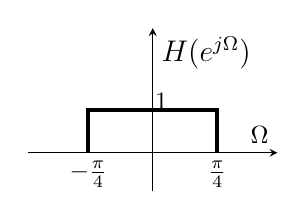
\begin{tikzpicture}[scale=0.9,transform shape]
    \begin{axis}[
        x=0.05\textwidth,y=0.05\textwidth,
        axis y line=center,
        axis x line=middle,
        xlabel=$\Omega$,ylabel={\large $H(e^{j\Omega})$},
        xmin=-2.9,xmax=2.9,
        ymin=-0.9,ymax=2.9,
        ticks=none
        ]
        \addplot[
        black,
        ultra thick
        ] coordinates {
            (-1.5,0) (-1.5,1) (1.5,1) (1.5,0)
        } ;
        \node at (-1.5,-.5) {$-\frac{\pi}{4}$};
        \node at (1.5,-.5) {$\frac{\pi}{4}$};
        \node at (0.2,1.2) {1} ;
    \end{axis} 
    \end{tikzpicture} & \hfill &
    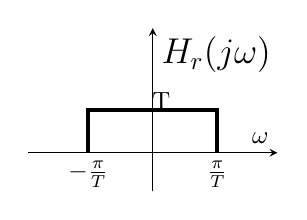
\begin{tikzpicture}[scale=0.9,transform shape]
    \begin{axis}[
        x=0.05\textwidth,y=0.05\textwidth,
        axis y line=center,
        axis x line=middle,
        xlabel=$\omega$,ylabel={\Large $H_r(j\omega)$},
        xmin=-2.9,xmax=2.9,
        ymin=-0.9,ymax=2.9,
        ticks=none
        ]
        \addplot[
        black,
        ultra thick
        ] coordinates {
            (-1.5,0) (-1.5,1) (1.5,1) (1.5,0)
        } ;
        \node at (-1.5,-.5) {$-\frac{\pi}{T}$};
        \node at (1.5,-.5) {$\frac{\pi}{T}$};
        \node at (0.2,1.2) {T} ;
    \end{axis} 
    \end{tikzpicture}
\end{tabular}